\newsheet{Day 2: Lattice Basis Reduction}{3}{2}
\vspace{-10pt}
\begin{center}
	\textbf{Given a basis, what are the shortest vectors}
	
	\textbf{in the lattice generated by this basis?}
\end{center}

The main reason $\{\u,\v\}=\{(1,0),\,(0,1)\}$ is so nice to work with is because it's an \emph{orthogonal} basis. This means that we can just compute the lengths of lattice points using the Pythagorean Theorem: when $\u$ and $\v$ are orthogonal, we have
\[\|a\u+b\v\|^2=a^2\|\u\|^2+b^2\|\v\|^2,\]
where $\|\cdot\|$ denotes taking the length of the vector. This implies that, unlike for some bases, there are no ``surprise'' short vectors; the only short vectors are those with small coefficients for $\u$ and $\v$.

Unfortunately, most lattices will not have orthogonal bases. But we can try to get as close as possible!

\section*{Attempting Orthogonalization}

\begin{explor}
	For any integer $n$, prove that $\{\u,\v\}$ and $\{\u,\v+n\u\}$ generate the same lattice.
\end{explor}

This gives us a valuable tool for finding new bases: we can slide one basis vector along the direction of another basis vector. Doing this allows us to make the angle between the basis vectors closer to a right angle.

\begin{explor}\label{exp:samen}
	Show that the same integer $n$ solves both of the following problems:
	\begin{itemize}
		\item Find $n$ such that $\v+n\u$ is as short as possible.
		\item Find $n$ such that the angle between $\u$ and $\v+n\u$ is as close to $90^\circ$ as possible.
	\end{itemize}
\end{explor}

\answer{Law of sines}

\begin{defn}
	We will say that a $2$-dimensional basis $\{\u,\v\}$ is \textbf{reduced} if $\|\u\|\leq\|\v\|$ and\\ $\|\v\|\leq\|\v+n\u\|$ for all integers $n$.
\end{defn}

\begin{explor}\label{exp:drawregion}
	Suppose $\u=(1,0)$. Draw the region in $\R^2$ containing all vectors $\v$ such that $\{\u,\v\}$ is a reduced basis. What will the region look like if you choose a different vector $\u$?
\end{explor}

Reduced bases are almost as nice as orthogonal bases to work with. In particular, lengths are relatively predictable, and it is straightforward to find the shortest vectors:

\begin{explor}
	If $\{\u,\v\}$ is a reduced basis, prove that the squared length of any lattice vector $a\u+b\v$ is at least $\frac12(a^2\|\u\|^2+b^2\|\v\|^2)$. Use this to conclude that there is no nonzero lattice vector shorter than $\u$.
\end{explor}
\begin{explor}
	Describe an algorithm that takes a basis as input, and returns a reduced basis generating the same lattice. Why must your algorithm terminate?
\end{explor}

\begin{explor}
	The mayor of Skewvillle (see Figure~\ref{fig:skewv}) is embarking on a massive construction project which will involve laying an entirely new road system. She wants to preserve the locations of all the intersections, but wants to minimize travel time between nearby intersections. What directions should the new roads be built in?
\end{explor}

\begin{center}
	\begin{figure}[h]
		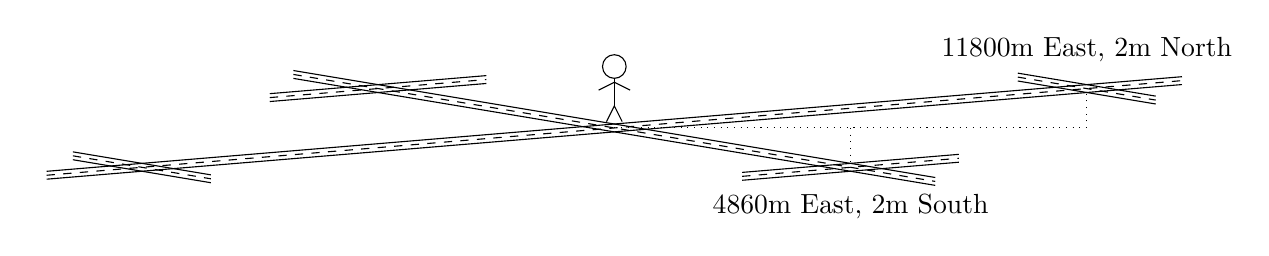
\begin{tikzpicture}
		
		\node (v1) at (-6-6/4.5,-0.5-0.5/4.5) {};
		\node (v2) at (6+6/4.5,0.5+0.5/4.5) {};
		\node (v3) at (-3-3/2.5,0.5+0.5/2.5) {};
		\node (v4) at (3+3/2.5,-0.5-0.5/2.5) {};
		\draw[dashed]  (v1) edge (v2);
		\draw[dashed]  (v3) edge (v4);
		\node at (6,1) {$11800$m East, $2$m North};
		\node at (3,-1) {$4860$m East, $2$m South};
		\draw[dotted] (0,0) -- (6,0);
		\draw[dotted] (6,0) -- (6,0.5);
		\draw[dotted] (3,0) -- (3,-0.5);
		
		\node (v1u) at (-6-6/4.5,-0.45-0.5/4.5) {};
		\node (v2u) at (6+6/4.5,0.55+0.5/4.5) {};
		\node (v1d) at (-6-6/4.5,-0.55-0.5/4.5) {};
		\node (v2d) at (6+6/4.5,0.45+0.5/4.5) {};
		\node (v3u) at (-3-3/2.5,0.45+0.5/2.5) {};
		\node (v4u) at (3+3/2.5,-0.55-0.5/2.5) {};
		\node (v3d) at (-3-3/2.5,0.55+0.5/2.5) {};
		\node (v4d) at (3+3/2.5,-0.45-0.5/2.5) {};
		\draw  (v1u) edge (v2u);
		\draw  (v1d) edge (v2d);
		\draw  (v3u) edge (v4u);
		\draw  (v3d) edge (v4d);
		
		\node (v5) at (6-3/3,0.5+0.5/3) {};
		\node (v6) at (6+3/3,0.5-0.5/3) {};
		\draw[dashed]  (v5) edge (v6);
		\node (v5u) at (6-3/3,0.5+0.5/3-0.05) {};
		\node (v6u) at (6+3/3,0.5-0.5/3-0.05) {};
		\node (v5d) at (6-3/3,0.5+0.5/3+0.05) {};
		\node (v6d) at (6+3/3,0.5-0.5/3+0.05) {};
		\draw  (v5u) edge (v6u);
		\draw  (v5d) edge (v6d);
		
		\node (v5) at (-6-3/3,-0.5+0.5/3) {};
		\node (v6) at (-6+3/3,-0.5-0.5/3) {};
		\draw[dashed]  (v5) edge (v6);
		\node (v5u) at (-6-3/3,-0.5+0.5/3-0.05) {};
		\node (v6u) at (-6+3/3,-0.5-0.5/3-0.05) {};
		\node (v5d) at (-6-3/3,-0.5+0.5/3+0.05) {};
		\node (v6d) at (-6+3/3,-0.5-0.5/3+0.05) {};
		\draw  (v5u) edge (v6u);
		\draw  (v5d) edge (v6d);
		
		\node (v5) at (3-6/4,-0.5-0.5/4) {};
		\node (v6) at (3+6/4,-0.5+0.5/4) {};
		\draw[dashed]  (v5) edge (v6);
		\node (v5u) at (3-6/4,-0.5-0.5/4-0.05) {};
		\node (v6u) at (3+6/4,-0.5+0.5/4-0.05) {};
		\node (v5d) at (3-6/4,-0.5-0.5/4+0.05) {};
		\node (v6d) at (3+6/4,-0.5+0.5/4+0.05) {};
		\draw  (v5u) edge (v6u);
		\draw  (v5d) edge (v6d);
		
		\node (v5) at (-3-6/4,0.5-0.5/4) {};
		\node (v6) at (-3+6/4,0.5+0.5/4) {};
		\draw[dashed]  (v5) edge (v6);
		\node (v5u) at (-3-6/4,0.5-0.5/4-0.05) {};
		\node (v6u) at (-3+6/4,0.5+0.5/4-0.05) {};
		\node (v5d) at (-3-6/4,0.5-0.5/4+0.05) {};
		\node (v6d) at (-3+6/4,0.5+0.5/4+0.05) {};
		\draw  (v5u) edge (v6u);
		\draw  (v5d) edge (v6d);
		
		\draw  (-0.5/5,0.08) --  (0,1/5+0.08) -- (0.5/5,0.08);
		\draw  (0,1/5+0.08) -- (0,3.5/5+0.08);
		\draw  (0,2.5/5+0.08) -- (-1/5,2/5+0.08);
		\draw  (0,2.5/5+0.08) -- (1/5,2/5+0.08);
		\draw[fill=white]  (0,3.5/5+0.08) ellipse (0.75/5 and 0.75/5);
		\end{tikzpicture}
		\caption{You and adjacent intersections (not to scale).}
		\label{fig:skewv}
	\end{figure}
\end{center}
\pagebreak
Unfortunately, if we try and extend this definition of ``reduced'' in a natural way to higher dimensions, things aren't as nice.

\begin{explor}\label{exp:3dbadbasis}
	Consider the basis
	\[\b_1=\begin{pmatrix}
	1\\0\\-10^{-6}
	\end{pmatrix},\,\b_2=\begin{pmatrix}
	1/2 \\ \sqrt{3}/2 \\ 2\cdot 10^{-6}
	\end{pmatrix},\,\b_3=\begin{pmatrix}
	-1/2 \\ \sqrt{3}/2 \\ -3\cdot 10^{-6}
	\end{pmatrix}\]
	(written as column vectors). Show that each pair of basis vectors is reduced, but that the lattice generated by $\{\b_1,\b_2,\b_3\}$ contains a vector that is much shorter than any of the basis vectors.
\end{explor}

\begin{explor}[(Optional)]
	We've shown that every $2$-D lattice has at least one reduced basis. In fact there will always be more than one (for example, if $\{\u,\v\}$ is a reduced basis then so is $\{\pm\u,\pm\v\}$).
	Add some extra constraints to the definition of ``reduced'' in order to guarantee that every lattice has \emph{exactly one} reduced basis \color{DarkGreen}
	
	(Hint: use the drawing from Exploration~\ref{exp:drawregion}. Which choices of $\v$ will generate the same lattice? How will you pin down a specific choice for the vector $\u$? Be especially careful of the situation in which there are more than two vectors with the same shortest length)
\end{explor}

\pagebreak

\section*{Optional Exploration: Short Vectors in Number Theory}

The problem of finding short vectors in a lattice has many applications. We'll explore a few of them here:

\begin{explor}
	Consider the lattice generated by the basis
	\[\u=\begin{pmatrix}
	1071\\0
	\end{pmatrix},\,\v=\begin{pmatrix}
	462 \\ 0.0001
	\end{pmatrix}.\]
	Explain why the reduced basis has the form
	\[\begin{pmatrix}
	0\\\text{[small]}
	\end{pmatrix},\,\begin{pmatrix}
	\gcd(1071,462) \\ \text{[small]}
	\end{pmatrix}.\]
\end{explor}

\begin{explor}
	Consider the lattice generated by
	\[\u=\begin{pmatrix}
	\pi\\0
	\end{pmatrix},\,\v=\begin{pmatrix}
	1 \\ 0.0001
	\end{pmatrix}.\]
	If you can find a short lattice vector $a\u+b\v$, explain how this gives you a rational approximation to $\pi$. What could you change about the basis in order to find better approximations?
\end{explor}

\begin{explor}\label{exp:polyroot}
	Suppose we have a real number $\alpha$ that we believe is the root of some quadratic polynomial, but all we know is a decimal approximation: $\alpha\approx 0.4708709$. Explain how finding a short vector in the lattice generated by
	\[\u=\begin{pmatrix}
	1\\0\\0
	\end{pmatrix},\,\v=\begin{pmatrix}
	0.4708709 \\ 0.0000001 \\ 0
	\end{pmatrix},\,\w=\begin{pmatrix}
	0.4708709^2 \\ 0\\ 0.0000001
	\end{pmatrix}.\]
	can be used to find a candidate for the mystery polynomial.
\end{explor}

\begin{comment}
\section*{OLD}

We'll continue to use $\R^2$ for motivation (keep using \url{https://stanford.edu/~jonlove/lattice-play.html}!), but with not much extra work we can say things about higher-dimensional lattices too. Let's start by generalizing some of the definitions from yesterday:

\begin{itemize}
	\item A set of $n$ vectors $\v_1,\ldots,\v_n\in\R^n$ is called a \textbf{\color{magenta}basis} if any vector in $\R^n$ can be written in the form $r_1\v_1+\cdots+r_n\v_n$ for exactly one choice of real numbers $r_1,\ldots,r_n$.
	\item Given a {\color{magenta}basis $\{\v_1,\ldots,\v_n\}$}, the \textbf{\color{gray} lattice generated by this basis} is the set of vectors
	\[\{a_1\v_1+a_2\v_2+\cdots+a_n\v_n\mid a_1,a_2,\ldots,a_n\in \Z\}.\]
	\item The {\color{magenta}fundamental parallelepiped of the basis} is the set of vectors
	\[\{r_1\v_1+r_2\v_2+\cdots+r_n\v_n\mid r_1,r_2,\ldots,r_n\in [0,1)\}.\]
\end{itemize}
We will also start to use matrices to describe lattices and their bases
\begin{itemize}
	\item The \textbf{\color{magenta}basis matrix $B$ of the basis $\{\v_1,\ldots,\v_n\}$} is the $n\times n$ matrix which has the basis vector $\v_i$ as the $i^{\text{th}}$ column:
	\[B=\begin{pmatrix}
	\mid & \mid & & \mid\\
	\v_1 & \v_2 & \cdots & \v_n\\
	\mid & \mid & & \mid	
	\end{pmatrix}=\begin{pmatrix}
	v_{11} & v_{21} & \cdots & v_{n1}\\
	v_{12} & v_{22} & \cdots & v_{n2}\\
	\vdots & \vdots & \ddots & \vdots\\
	v_{1n} & v_{2n} & \cdots & v_{nn}\\
	\end{pmatrix}.\]
	A basis matrix will always be invertible\footnote{A matrix $M$ is invertible if there exists a matrix $M^{-1}$ with the property that $MM^{-1}$ is the identity matrix ($1$s on the top-left-to-bottom-right diagonal, and $0$s everywhere else).} (Exploration~\ref{exp:basisinv}).
	\item $M_n(\Z)$ is the set of all $n\times n$ matrices with integer entries.
	\item $\GL_n(\Z)$ is the set of matrices in $M_n(\Z)$ with an inverse matrix which is also in $M_n(\Z)$.
\end{itemize}
\noindent
A word of warning: we will be using matrices in more than one way. The first way is to store a list of vectors (basis matrices); the entries do not need to be integers in this case. But we will also use matrices as \emph{operations} on these sets of vectors (Exploration~\ref{exp:changebasis}).

\begin{explor}
	Become convinced that any basis matrix is, in fact, invertible. \color{DarkGreen}(Hint: Think of the matrix as a linear map. What does it do to vectors in the standard basis?)
\end{explor}

\begin{explor}\label{exp:ingl2ornot}
	Show that $\begin{psmallmatrix}
	3 & 5\\1&2
	\end{psmallmatrix}\in \GL_2(\Z)$, but $\begin{psmallmatrix}
	3 & 6\\1&2
	\end{psmallmatrix}$ and $\begin{psmallmatrix}
	3 & 4\\1&2
	\end{psmallmatrix}$ are not in $\GL_2(\Z)$. Come up with some other examples of matrices in $\GL_2(\Z)$, and matrices in $M_2(\Z)$ that are not in $\GL_2(\Z)$. (Do you have any guesses for a criterion that can be used to tell the two cases apart?)
\end{explor}

\begin{explor}\label{exp:changebasis}
	Using the lattice player, pick a basis $\{\u,\v\}$ of your choice. What is the corresponding basis matrix $B$?
	
	Now for various choices of $C\in M_2(\Z)$ (try the matrices from Exploration \ref{exp:ingl2ornot}), compute the product matrix $BC$. Describe the columns of this matrix --- can you identify where they appear in the lattice player?
\end{explor}

\begin{explor}
	Prove the following proposition. (You may not have time to prove it in class; I encourage you to work out the details afterwards.)
\end{explor}

\begin{toprove}{Proposition}
	Suppose $B$ and $B'$ are two $n\times n$ basis matrices. Then $B$ and $B'$ generate the same lattice if and only if there exists $C\in\GL_n(\Z)$ such that $B'=BC$.
\end{toprove}

\section*{Classifying $2$-D Lattices}

We've seen that a single lattice can be represented by many different bases. Our goal now is to find a ``best possible'' basis for any given lattice. 

Let $\LL$ be a lattice generated by vectors $\u$ and $\v$.

\begin{explor}
	If $a$ and $b$ are relatively prime, prove that there exists a basis of $\LL$ with $a\u+b\v$ as one of the basis vectors. 
\end{explor}

\begin{explor}\label{exp:chooseshort}
	Let $\p\in\LL$ be a nonzero vector such that no shorter nonzero lattice point exists. Prove that there is a basis generating $\LL$ that contains $\p$.
\end{explor}

We can now replace $\{\u,\v\}$ with a different basis for $\LL$. By Exploration~\ref{exp:chooseshort}, we can assume $\u$ is one of the shortest nonzero vectors in $\LL$. We can now scale and rotate the entire plane so that $\u$ is sent to $(1,0)$ (this changes the lattice itself, not just the basis, so we'll have to keep track of this later); by replacing $\v$ with $-\v$ if necessary, we can assume $\v$ is in the upper half plane.

\begin{explor}
	Prove that for any integer $n$, $\{\u,\v\}$ and $\{\u,\v+n\u\}$ generate the same lattice. If $\u=(1,0)$, conclude that we can take $\v$ to have $x$-coordinate in $(-\frac12, \frac12]$. What else can we say about this choice of $\v$? Complete Theorem~\ref{thm:2dclass}, draw/visualize the region that $\v$ can lie in, and prove the result.
\end{explor}

\begin{toprove}{Theorem}\label{thm:2dclass}
	Any lattice in $\R^2$ can be obtained by applying scaling and rotation to a lattice generated by $\{(1,0),\v\}$, where $\v$ is in the following region of the plane:
	
	\vspace{20pt}
	
	\centering
	\underline{\hspace{200pt}}
\end{toprove}

\section*{Optional Exploration: Filling the Gaps}

\begin{explor}
	Given a matrix in $M_n(\Z)$, prove that it is in $\GL_n(\Z)$ if and only if its determinant equals $\pm 1$.
\end{explor}

\begin{explor}
	In order to complete the classification of $2$-d lattices, we need to show that any lattice produces a \emph{unique} choice of $\v$ in Theorem~\ref{thm:2dclass}. Prove that if $\v$ and $\v'$ are distinct points in the given region, then the lattices generated by $\{(1,0),\v\}$ and by $\{(1,0),\v'\}$ are not related to each other by any scaling or rotation. \color{DarkGreen}(You may need to modify the region slightly --- be careful about what happens when $\v$ is on the unit circle!)
\end{explor}




how close can we get?

\begin{explor}
Let $\theta$ denote the angle between $\u$ and $\v$. Find a condition on $\theta$ that will guarantee that the length of $a\u+b\v$ is at least $\frac12(a^2\|u\|^2+b^2\|v\|^2)$.

\color{DarkGreen}(Hint: The vector addition of $a\u$ and $b\v$ makes a triangle; apply the law of cosines)
\end{explor}

If a basis has an angle $\theta$ in this range, we will call it ``near-orthogonal.''

\begin{explor}\label{exp:noshorter}
If $\{\u,\v\}$ is near-orthogonal, prove that the lattice they generate has no nonzero vectors shorter than both $\u$ and $\v$. 
\end{explor}

Near-orthogonal bases are relatively easy to work with, because lengths of vectors behave in predictable ways (there are no surprise short vectors). So it would be great if we had a method to take non-orthogonal bases and make them closer to orthogonal.

\end{comment}
